%!TEX output_directory = aux
%!TEX aux_directory = aux

\documentclass[10pt]{beamer}

\usetheme[
  numbering=fraction,
  block=fill,
  % background=dark
  ]{metropolis}

\usepackage{appendixnumberbeamer}
\usepackage{booktabs}
\usepackage[scale=2]{ccicons}
%\usepackage{pgfplots}
%\usepgfplotslibrary{dateplot}

\usepackage[absolute,overlay]{textpos}
\setlength{\TPHorizModule}{\paperwidth}
\setlength{\TPVertModule}{\paperheight}

% ------------------------ %
% 	  Packages		%
% ------------------------ %

\usepackage[utf8]{inputenc}
\usepackage[T1]{fontenc}
\usepackage{xparse}
\usepackage{pgffor}
\usepackage{ifthen}
\usepackage{xspace}
\usepackage{xcolor}
\usepackage{amsmath}
\usepackage{amssymb}
\usepackage{amsfonts}
\usepackage{amsthm}
\usepackage{mathrsfs}
\usepackage{bbm}
\usepackage{mathtools}
\usepackage{stmaryrd}
\usepackage[ruled,linesnumbered]{algorithm2e}
\newcommand\mycommfont[1]{\footnotesize\ttfamily\textcolor{blue}{#1}}
\SetCommentSty{mycommfont}
\usepackage{csquotes}
\usepackage{dblfloatfix}
\usepackage{comment}
\renewcommand{\ttdefault}{lmtt}


% ------------------------ %
% 	  Shortcuts		  %
% ------------------------ %

% Lowercase styles
\foreach \x in {a,...,z}{%
	\expandafter\xdef\csname \x\endcsname{\noexpand\ensuremath{\noexpand\mathbf{\x}}}
}
\foreach \x in {a,...,z}{%
	\expandafter\xdef\csname \x rm\endcsname{\noexpand\ensuremath{\noexpand\mathrm{\x}}}
}

% Uppercase styles
\foreach \x in {A,...,Z}{%
	\expandafter\xdef\csname \x\endcsname{\noexpand\ensuremath{\noexpand\mathbf{\x}}}
}
\foreach \x in {A,...,Z}{%
	\expandafter\xdef\csname \x rm\endcsname{\noexpand\ensuremath{\noexpand\mathrm{\x}}}
}
\foreach \x in {A,...,Z}{%
	\expandafter\xdef\csname \x bb\endcsname{\noexpand\ensuremath{\noexpand\mathbb{\x}}}
}
\foreach \x in {A,...,Z}{%
	\expandafter\xdef\csname \x c\endcsname{\noexpand\ensuremath{\noexpand\mathcal{\x}}}
}

% Figures styles
\def\0{{\mathbf 0}}
\def\1{{\mathbf 1}}

% Miscellaneous
\def\ie{\textit{i.e.}}
\def\eg{\textit{e.g.}}
\def\etal{\textit{et al.}}
\def\resp{\textit{resp.}}

% Notes
\def\addNote#1{{\noindent\color{blue}{[Note : #1]}}}
\def\toDo#1{{\noindent\color{red}{[Todo : #1]}}}
\def\addCite{{\noindent\color{orange}{[Cite] }}}

% Fonts
\newcommand{\fontpb}[1]{\mathcal{#1}}
\newcommand{\fontobj}[1]{#1}
\newcommand{\fontset}[1]{\mathcal{#1}}
\newcommand{\fontfunc}[1]{\mathrm{#1}}
\newcommand{\fontregion}[1]{\mathbb{#1}}

% Problem data
\newcommand{\sparsitylevel}{k}
\newcommand{\pdim}{n}
\newcommand{\ddim}{m}
\newcommand{\obs}{\y}
\newcommand{\dic}{\A}
\newcommand{\atom}{\a}
\newcommand{\regone}{\lambda}
\newcommand{\regtwo}{\gamma}
\newcommand{\matred}{\B}
\newcommand{\vecred}{\b}
\newcommand{\matnorm}{\M}

% Problems
\newcommand{\Primalletter}{P}
\newcommand{\Dualletter}{D}
\newcommand{\primalletter}{p}
\newcommand{\dualletter}{d}
\newcommand{\ppb}{\fontpb{\Primalletter}}
\newcommand{\dpb}{\fontpb{\Dualletter}}
\newcommand{\pfunc}{\fontfunc{\Primalletter}}
\newcommand{\dfunc}{\fontfunc{\Dualletter}}
\newcommand{\pobj}{\opt{\primalletter}}
\newcommand{\dobj}{\opt{\dualletter}}
\newcommand{\reform}[2]{#1_{#2}}
		
% Variables
\newcommand{\pvletter}{x}
\newcommand{\dvletter}{u}
\newcommand{\svletter}{\theta}
\newcommand{\pv}{\mathbf{\pvletter}}
\newcommand{\dv}{\mathbf{\dvletter}}
\newcommand{\sv}{\boldsymbol{\svletter}}
\newcommand{\pve}[1]{\pv(#1)}
\newcommand{\dve}[1]{\dv(#1)}
\newcommand{\sve}[1]{\sv(#1)}
\newcommand{\pvopt}{\opt{\pv}}
\newcommand{\dvopt}{\opt{\dv}}
\newcommand{\pvopte}[1]{\pvopt(#1)}
\newcommand{\dvopte}[1]{\dvopt(#1)}

% Screening
\newcommand{\idx}{i}
\newcommand{\idxscreen}{i}
\newcommand{\setind}{\fontset{S}}
\newcommand{\setpos}{\setind_+}
\newcommand{\setneg}{\setind_-}
\newcommand{\setnul}{\setind_0}
\newcommand{\setund}{\setdef_*}
\newcommand{\setposneg}{\setind_{\pm}}
\newcommand{\setdef}{\setind}
\newcommand{\setposopt}{\opt{\setpos}}
\newcommand{\setnegopt}{\opt{\setneg}}
\newcommand{\setnulopt}{\opt{\setnul}}
\newcommand{\safesphere}{\fontregion{S}}
\newcommand{\spherecenter}{\c}
\newcommand{\sphereradius}{r}
\newcommand{\lipschitz}{L}


% Operators
\newcommand{\abs}[1]{|#1|}
\newcommand{\argmin}{\mathrm{argmin}}
\newcommand{\argmax}{\mathrm{argmax}}
\newcommand{\clip}[3]{\mathrm{clip}_{\kintervcc{#2}{#3}}(#1)}
\newcommand{\card}[1]{|#1|}
\newcommand{\conj}[1]{#1^*}
\newcommand{\eigval}{\sigma}
\newcommand{\gap}{\mathrm{gap}}
\newcommand{\grad}{\nabla}
\newcommand{\subdiff}{\partial}
\newcommand{\Icvx}{\eta}
\newcommand{\Id}{\I}
\newcommand{\intervint}[2]{\llbracket#1,#2\rrbracket}
\newcommand{\norm}[2]{\|#1\|_#2}
\newcommand{\opt}[1]{#1^{\star}}
\newcommand{\scalprod}[2]{\langle{#1,#2}\rangle}
\newcommand{\sign}[1]{\mathrm{sign}({#1})}
\newcommand{\softhresh}[2]{\Tc(#1,#2)}
\newcommand{\relu}[1]{[#1]_+}
\newcommand{\transp}[1]{#1^{\mathrm{T}}}
\newcommand{\complset}[1]{#1^{\complement}}
\newcommand{\reduced}[1]{\tilde{#1}}

\DeclarePairedDelimiter\ceil{\lceil}{\rceil}
\DeclarePairedDelimiter\floor{\lfloor}{\rfloor}

\usepackage{kmath}
\newcommand{\emphone}[1]{{\color{orange}#1}}
\newcommand{\emphtwo}[1]{{\color{teal}#1}}

\title{Screen \& Relax}
\subtitle{Accelerating the resolution of the Elastic-Net by safe identification of the solution support}
\date{ICASSP 2022}
\author{Theo Guyard${}^{\star}$, Cedric Herzet${}^{\dagger}$, Clement Elvira${}^{\ddagger}$}
\institute{
  \(^{\star}\) Univ Rennes, INSA Rennes, CNRS, IRMAR-UMR 6625, F-35000 Rennes, France \\ 
	\(^{\dagger}\) INRIA Rennes-Bretagne Atlantique, Campus de Beaulieu, 35000 Rennes, France \\ 
  \(^{\ddagger}\) SCEE/IETR UMR CNRS 6164, CentraleSupélec, 35510 Cesson Sévigné, France
}

\begin{document}

\begin{frame}[plain]
  \maketitle
\end{frame}

\begin{frame}{Table of contents}
  \setbeamertemplate{section in toc}[sections numbered]
  \tableofcontents[hideallsubsections]
\end{frame}

\section{The Elastic-Net problem}

\begin{frame}{Sparse-linear problem}
  \textbf{Ingredients :}
  \begin{itemize}
    \item An \emphone{observation} $\obs \in \kR^{\ddim}$
    \item A \emphone{dictionary} $\dic=[\atom_{\idx}]_{\idx=1}^{\pdim} \in \kR^{\ddim\times\pdim}$ (columns $\equiv$ \emphone{atoms})
  \end{itemize}

  \pause

  \textbf{Objectives :}
  \begin{itemize}
    \item Approximate the \emphone{observation} as a linear combination of the \emphone{atoms}
    \item The linear combination must be \emph{sparse}
  \end{itemize}

  \pause

  \begin{center}
    \begin{minipage}{0.5\linewidth}
      \begin{block}{Problem}
        \centering
        Find $\pv$ \emph{sparse} such that $\obs \simeq \dic \pv$
      \end{block}
    \end{minipage}
  \end{center}

  \pause

  The vector $\pv$ weights each atom in the approximation.
\end{frame}

\begin{frame}{The Elastic-net problem}
  \textbf{Idea :} Consider the problem
  \begin{block}{Elastic-net}
    \begin{equation}
      \label{prob:primal}
      \pvopt = \argmin_{\pv} \ 
      \Big\{
      \pfunc(\pv) = 
        \tfrac{1}{2}\norm{\obs-\dic\pv}{2}^2
        + \regone \norm{\pv}{1}
        + \tfrac{\regtwo}{2} \norm{\pv}{2}^2
      \Big\}
      \tag{$\ppb$}
    \end{equation}
  \end{block}  
  where $\regone>0$ and $\regtwo>0$ are two hyperparameters. \\~\\

  \pause

  \textbf{Properties :}
  \begin{itemize}
    \item Ensures a good approximation
    \item Induces sparsity
    \item Good statistical properties
    \item Convex problem
  \end{itemize}
\end{frame}

\section{Screening and relaxing tests}

\begin{frame}{Main idea}
  \textbf{Sparse problem :}
  \begin{itemize}
    \item Where are \emphone{zero} entries of $\pvopt$ ?
    \item Where are \emphone{non-zero} entries of $\pvopt$ ?
  \end{itemize}

  \vspace{-0.25cm}
  \pause

  \begin{itemize}
    \item Can we accelerate solution methods using this knowledge ?
  
  \end{itemize}
  
  \vspace{-0.25cm}
  \pause

  \begin{itemize}
    \item[$\rightarrow$] Spoiler alert : yes !
    \item[$\rightarrow$] We can leverage \emphone{duality} and \emphone{optimality conditions}
  \end{itemize}

  \vspace{0.5cm}
  \pause


  \begin{block}{Fenchel dual of \eqref{prob:primal}}
  \begin{equation}
    \label{prob:dual}
      \dvopt = \argmax_{\dv} \ 
      \Big\{
        \dfunc(\dv) = 
        \tfrac{1}{2} \norm{\obs}{2}^2 
        - \tfrac{1}{2}\norm{\obs - \dv}{2}^2 
        -\tfrac{1}{2\regtwo}
        \|[\abs{\ktranspose{\dic}\dv} - \regone]_+\|_2^2
      \Big\}
      \tag{\(\Dc\)}
  \end{equation}
\end{block}
\end{frame}

\begin{frame}{Screening and relaxing tests}
  \textbf{Optimality conditions :}
  \begin{equation*}
    \begin{array}{rcl}
      \abs{\transp{\atom_{\idx}}\dvopt} \leq \regone &\iff& \pvopte{\idx} = 0 \\
      \abs{\transp{\atom_{\idx}}\dvopt} > \regone &\iff& \pvopte{\idx} \neq 0 
    \end{array}
  \end{equation*}

  \pause
  \begin{center}
    \rotatebox[origin=c]{-90}{\LARGE$\leadsto$}
  \end{center}
  \vspace{-0.2cm}

  \textbf{\emphone{Relaxed} optimality condition :} Let $\safesphere(\dv,\sphereradius)$ be a spherical region containing $\dvopt$, then
  \begin{equation*}
    \begin{array}{rcl}
      \abs{\transp{\atom_{\idx}}\dv} + \sphereradius < \regone &\implies& \pvopte{\idx} = 0 \qquad \text{\emphone{(screening test)}} \\
      \abs{\transp{\atom_{\idx}}\dv} - \sphereradius > \regone &\implies& \pvopte{\idx} \neq 0 \qquad \text{\emphone{(relaxing test)}} 
    \end{array}
  \end{equation*}
\end{frame}

% \begin{frame}{Screening and relaxing tests}
%   \begin{figure}
%     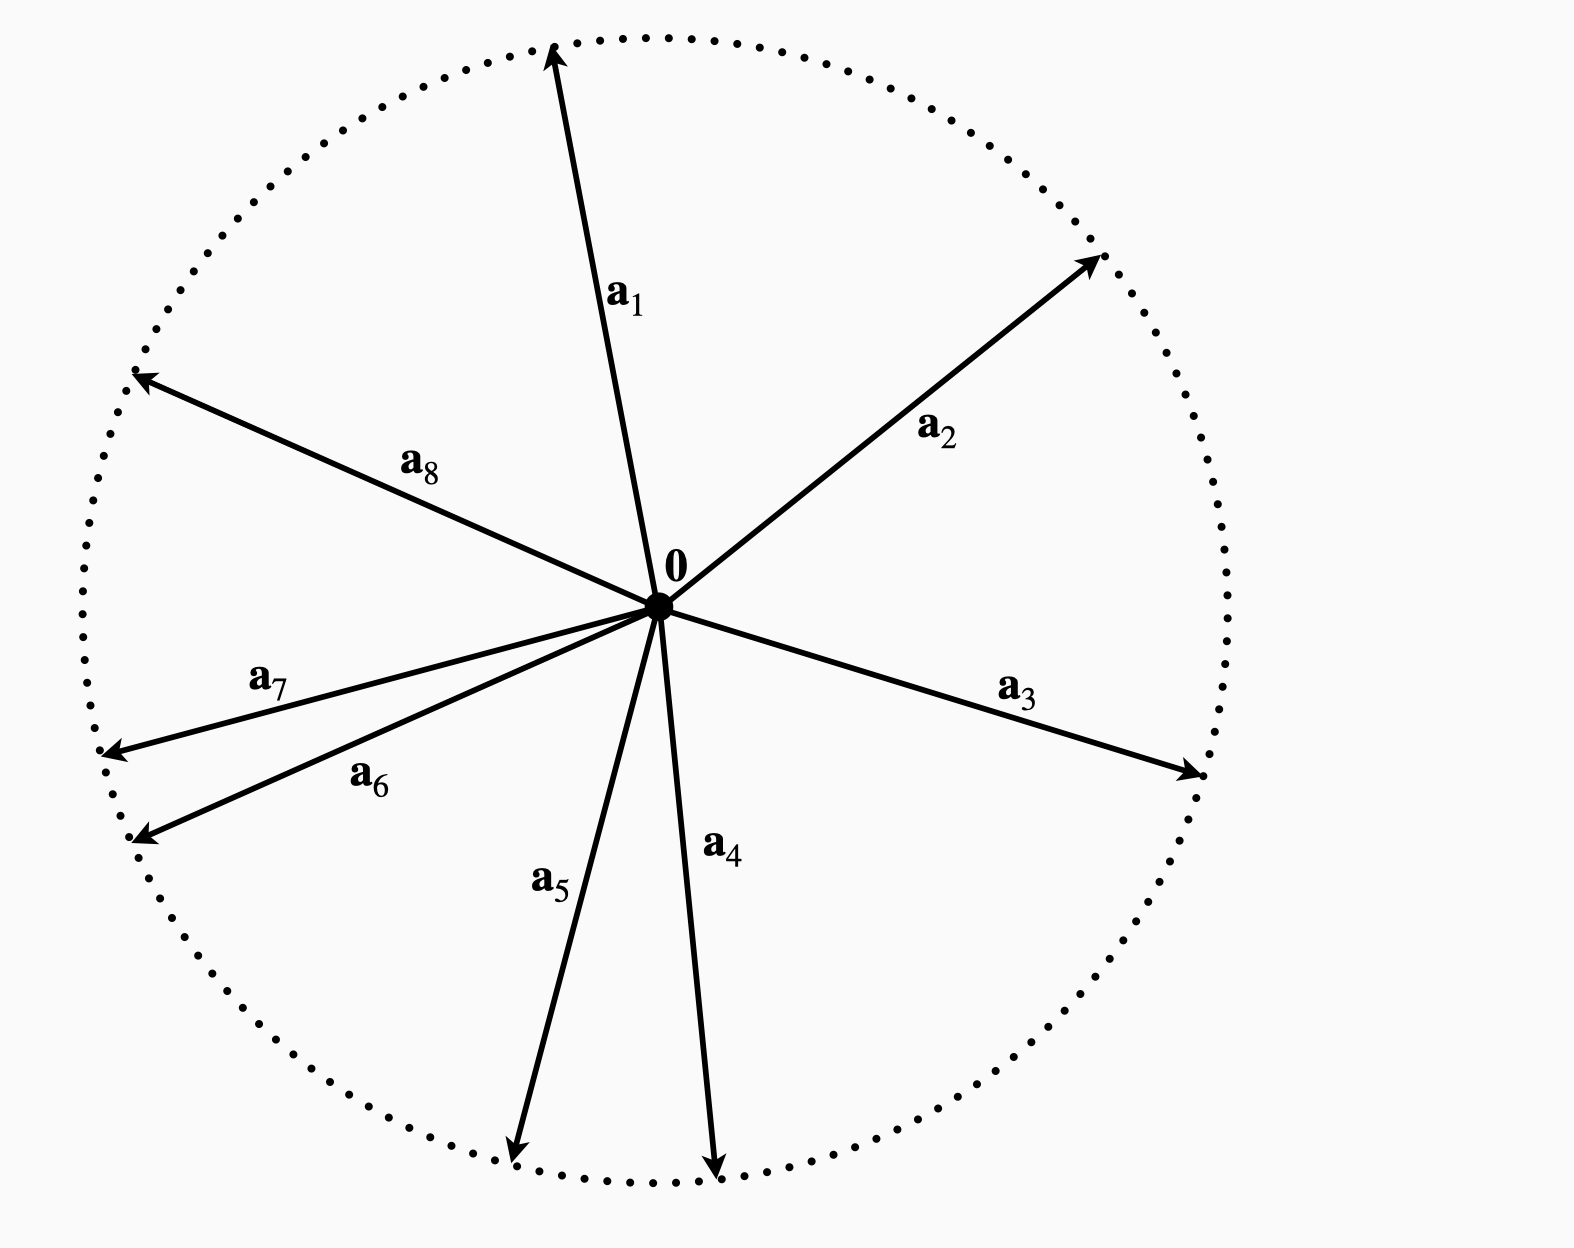
\includegraphics[width=0.8\linewidth]{img/1.png}
%   \end{figure}
% \end{frame}

% \begin{frame}{Screening and relaxing tests}
%   \begin{figure}
%     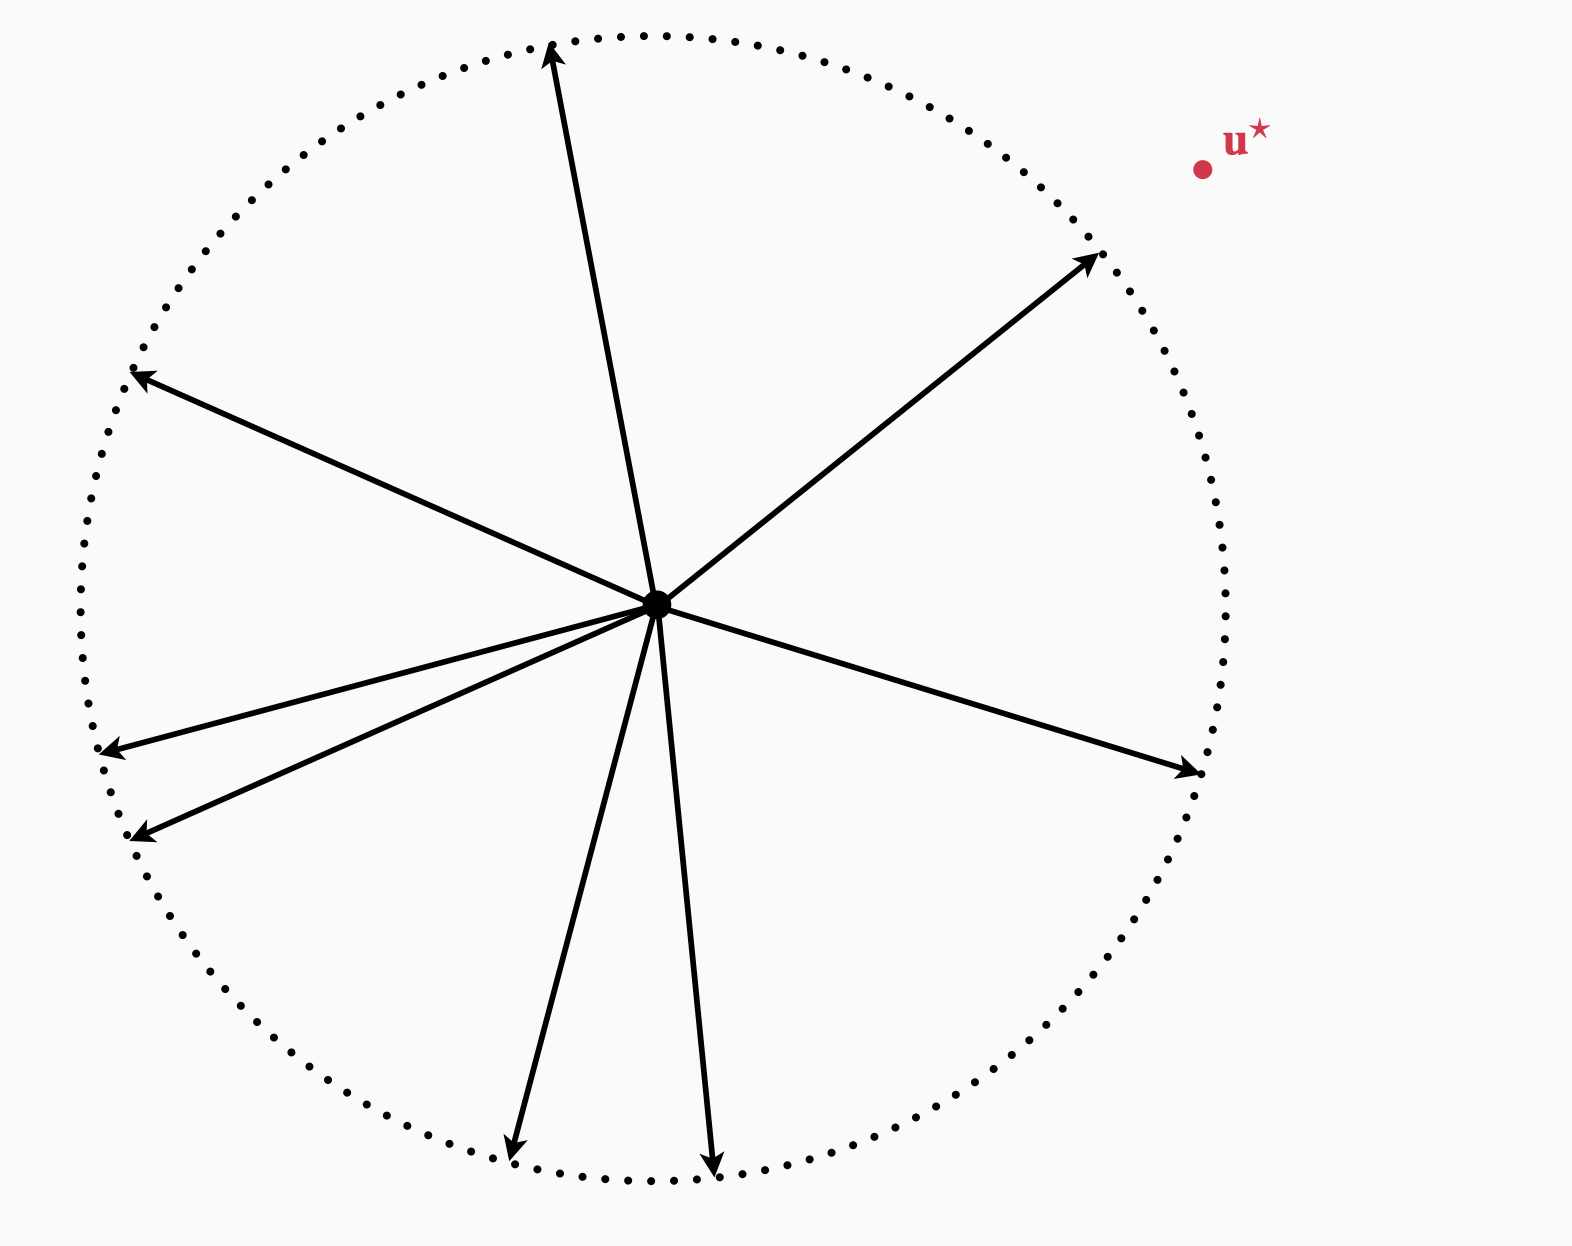
\includegraphics[width=0.8\linewidth]{img/2.png}
%   \end{figure}
% \end{frame}

% \begin{frame}{Screening and relaxing tests}
%   \begin{figure}
%     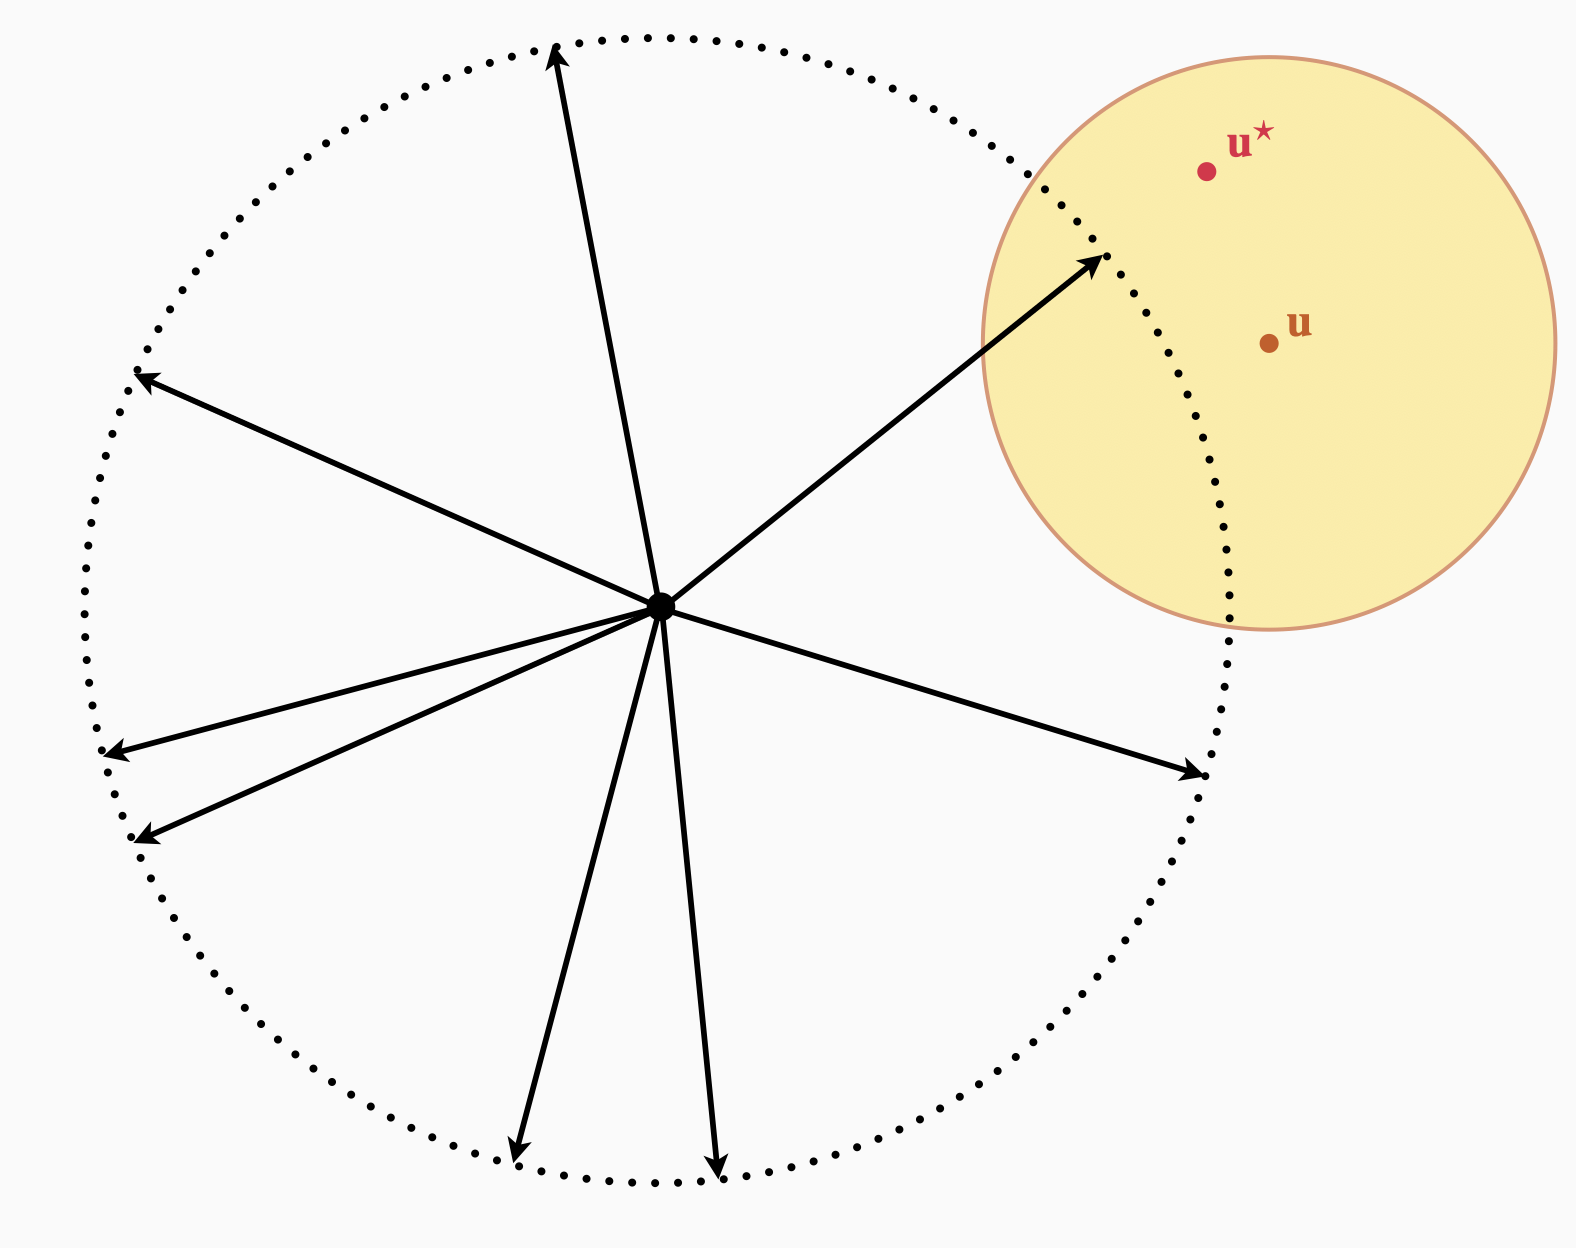
\includegraphics[width=0.8\linewidth]{img/3.png}
%   \end{figure}
% \end{frame}

% \begin{frame}{Screening and relaxing tests}
%   \begin{figure}
%     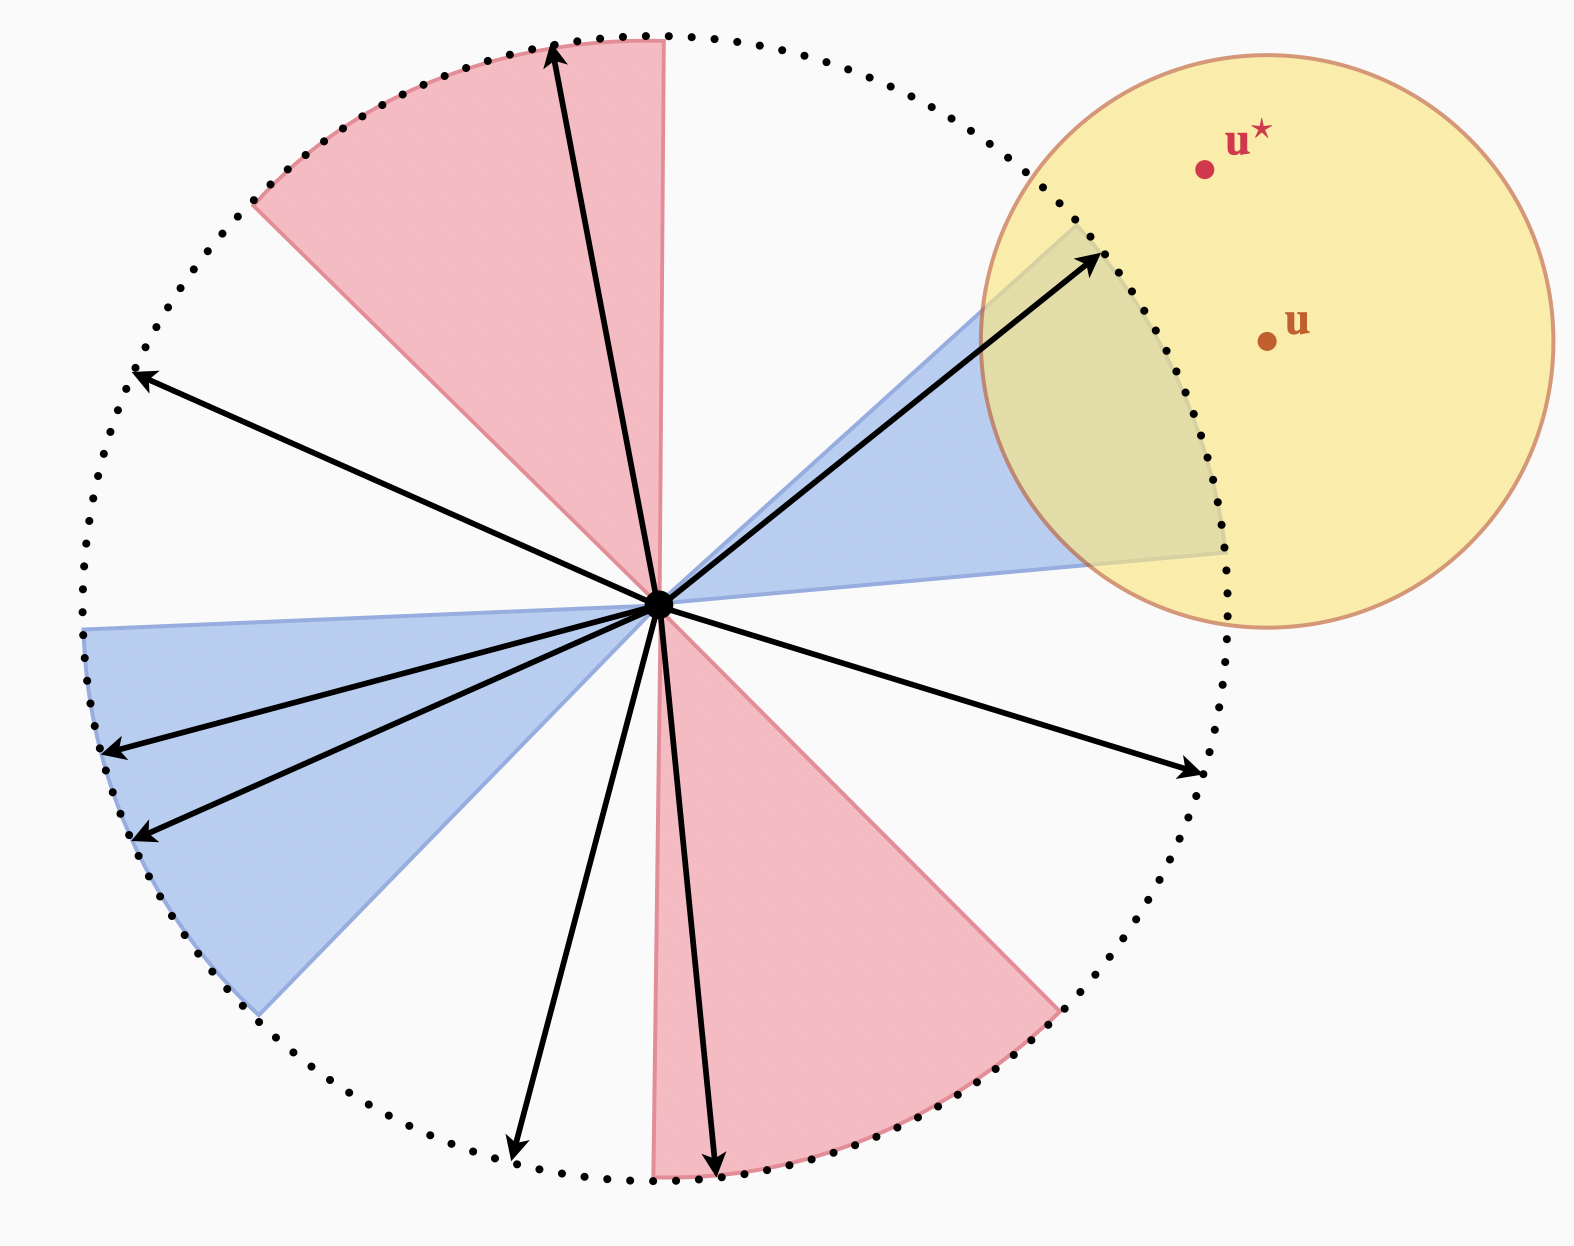
\includegraphics[width=0.8\linewidth]{img/4.png}
%   \end{figure}
% \end{frame}

% \begin{frame}{Screening and relaxing tests}
%   \begin{figure}
%     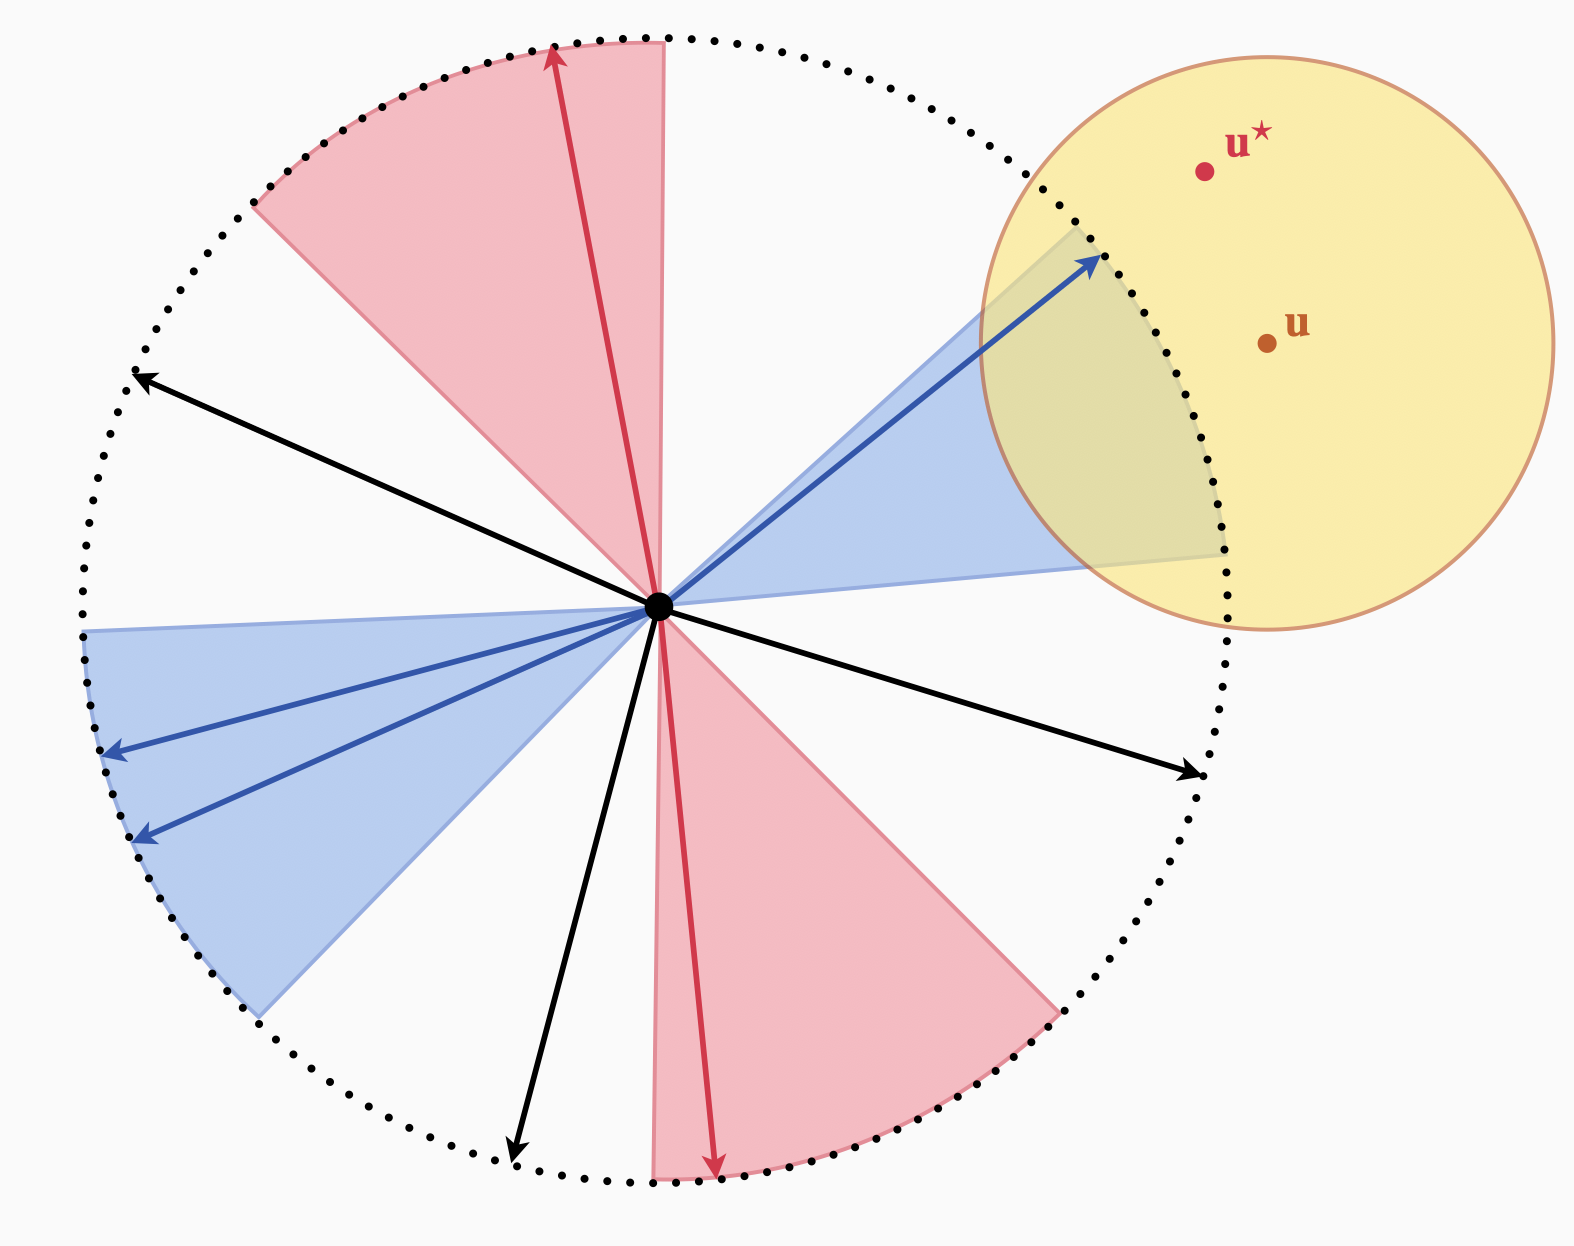
\includegraphics[width=0.8\linewidth]{img/5.png}
%   \end{figure}
% \end{frame}

\section{Dimensionality reduction}

\begin{frame}{Problem reduction}
  \begin{alertblock}{With screening test}
    \emphone{Zero} entries of $\pvopt$ can be \emphone{discarded} from the problem without changing the objective value.
  \end{alertblock}
  \vspace{1.5cm}

  \pause

  \begin{alertblock}{With relaxing test}
    \emphone{Nonzero} entries of $\pvopt$ can be expressed as a \emphone{linear combination} of all the other entries.
  \end{alertblock}
\end{frame}

\begin{frame}{Problem reformulation}
  \textbf{Let $(\setnul,\setposneg,\setund)$ be subsets of zero, non-zero and unclassified indices of $\pvopt$ :}
  \begin{equation*}
    \pvopt = \argmin_{\pv} \ 
    \Big\{
    \pfunc(\pv) = 
      \tfrac{1}{2}\norm{\emphone{\obs}-\emphone{\dic}\pv}{2}^2
      + \regone \norm{\pv}{1}
      + \tfrac{\regtwo}{2} \|\pv\|_{\emphone{2}}^2
    \Big\}
  \end{equation*}

  \pause
  \begin{center}
    Solve an $\pdim$ dimensional problem
  \end{center}

  \pause
  \vspace{-0.2cm}
  \begin{center}
    \vspace{0.1cm}
    \rotatebox[origin=c]{-90}{\LARGE$\leadsto$}
  \end{center}
  \vspace{-0.2cm}

  \begin{equation*}
    \begin{array}{rl}
      \pvopt_{\setund} &= \argmin_{\pv} \ 
      \Big\{
      \reduced{\pfunc}(\pv) = 
        \tfrac{1}{2}\norm{\emphone{\reduced{\obs}}-\emphone{\reduced{\dic}}\pv}{2}^2
        + \regone \norm{\pv}{1}
        + \tfrac{\regtwo}{2} \|\pv\|_{\emphone{\matnorm}}^2
      \Big\} \\
      \pvopt_{\setposneg} &= \matred\pvopt_{\setund} + \vecred \\
      \pvopt_{\setnul} &= \0
    \end{array}
  \end{equation*}

  \pause
  \begin{itemize}
    \item Compute $\reduced{\obs}$, $\reduced{\dic}$, $\matnorm$, $\matred$ and $\vecred$ (linear algebra operations)
    \item Solve an $\pdim-\card{\setnul}-\card{\setposneg}$ dimensional problem
  \end{itemize}
\end{frame}

\begin{frame}{Dynamic Screen \& Relax principle}
  \begin{figure}
    \centering
    \begin{minipage}{0.8\linewidth}
      \begin{algorithm}[H]
        \small
        \DontPrintSemicolon
        \SetKwInOut{Input}{Input}
        \Input{$\pv^{(0)}$, $\dic$, $\obs$, $\regone$, $\regtwo$}
        
        \BlankLine
        \((\setnul,\setposneg,\setund) \leftarrow (\emptyset,\emptyset,\{1,\dots,\pdim\})\)\;
        \BlankLine

        \While{convergence criterion is not met}{
          %
          Update the current iterate \;
          Compute a new safe sphere \;
          Update $(\setnul,\setposneg,\setund)$ with screening and relaxing tests\;
          Update the problem data\;
          \If{$\setund = \emptyset$}{
            The solution is available in closed form
          }
        }
        \caption{``Screen \& Relax'' solving procedure}
      \end{algorithm}
    \end{minipage}
  \end{figure}
\end{frame}

\section{Some numerical results}

\begin{frame}{Some numerical results}
  \textbf{Setup :} Percentage of instances solved up to a given accuracy for a fixed FLOPs budget.
  
  \pause
  \begin{figure}
    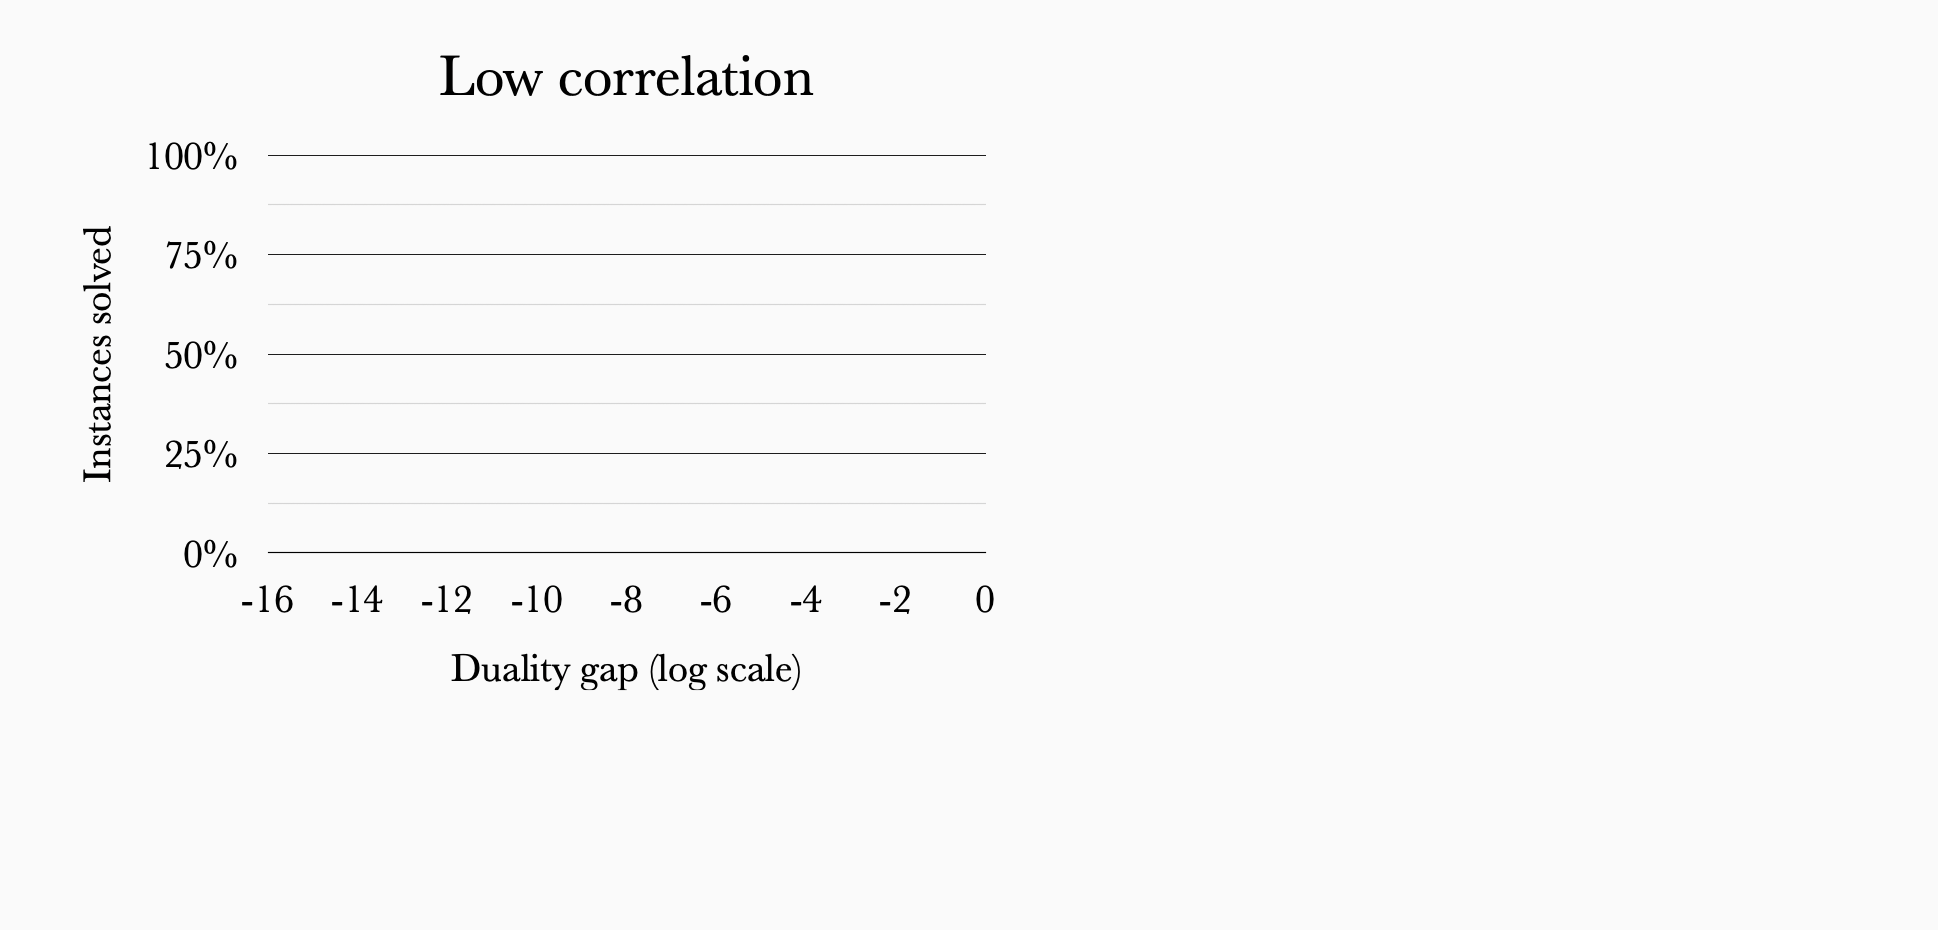
\includegraphics[width=\linewidth]{img/6.png}
  \end{figure}
\end{frame}

\begin{frame}{Some numerical results}
  \textbf{Setup :} Percentage of instances solved up to a given accuracy for a fixed FLOPs budget.
  \begin{figure}
    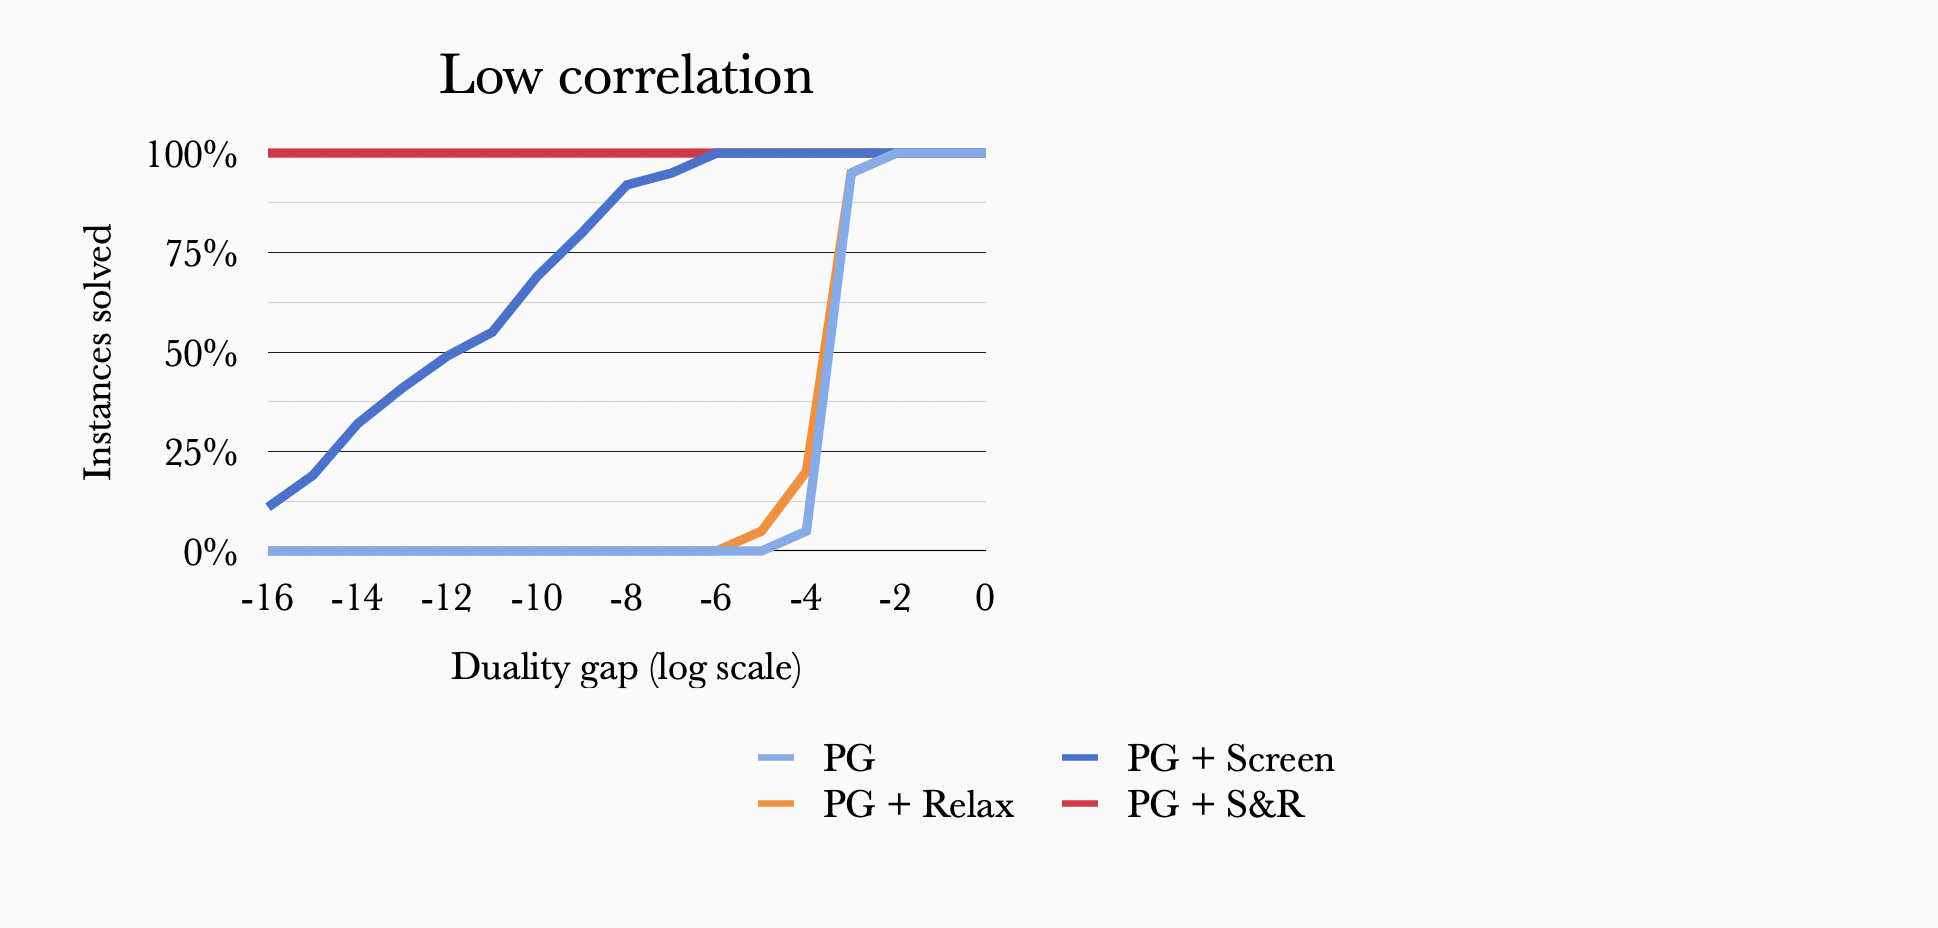
\includegraphics[width=\linewidth]{img/7.png}
  \end{figure}
\end{frame}

\begin{frame}{Some numerical results}
  \textbf{Setup :} Percentage of instances solved up to a given accuracy for a fixed FLOPs budget.
  \begin{figure}
    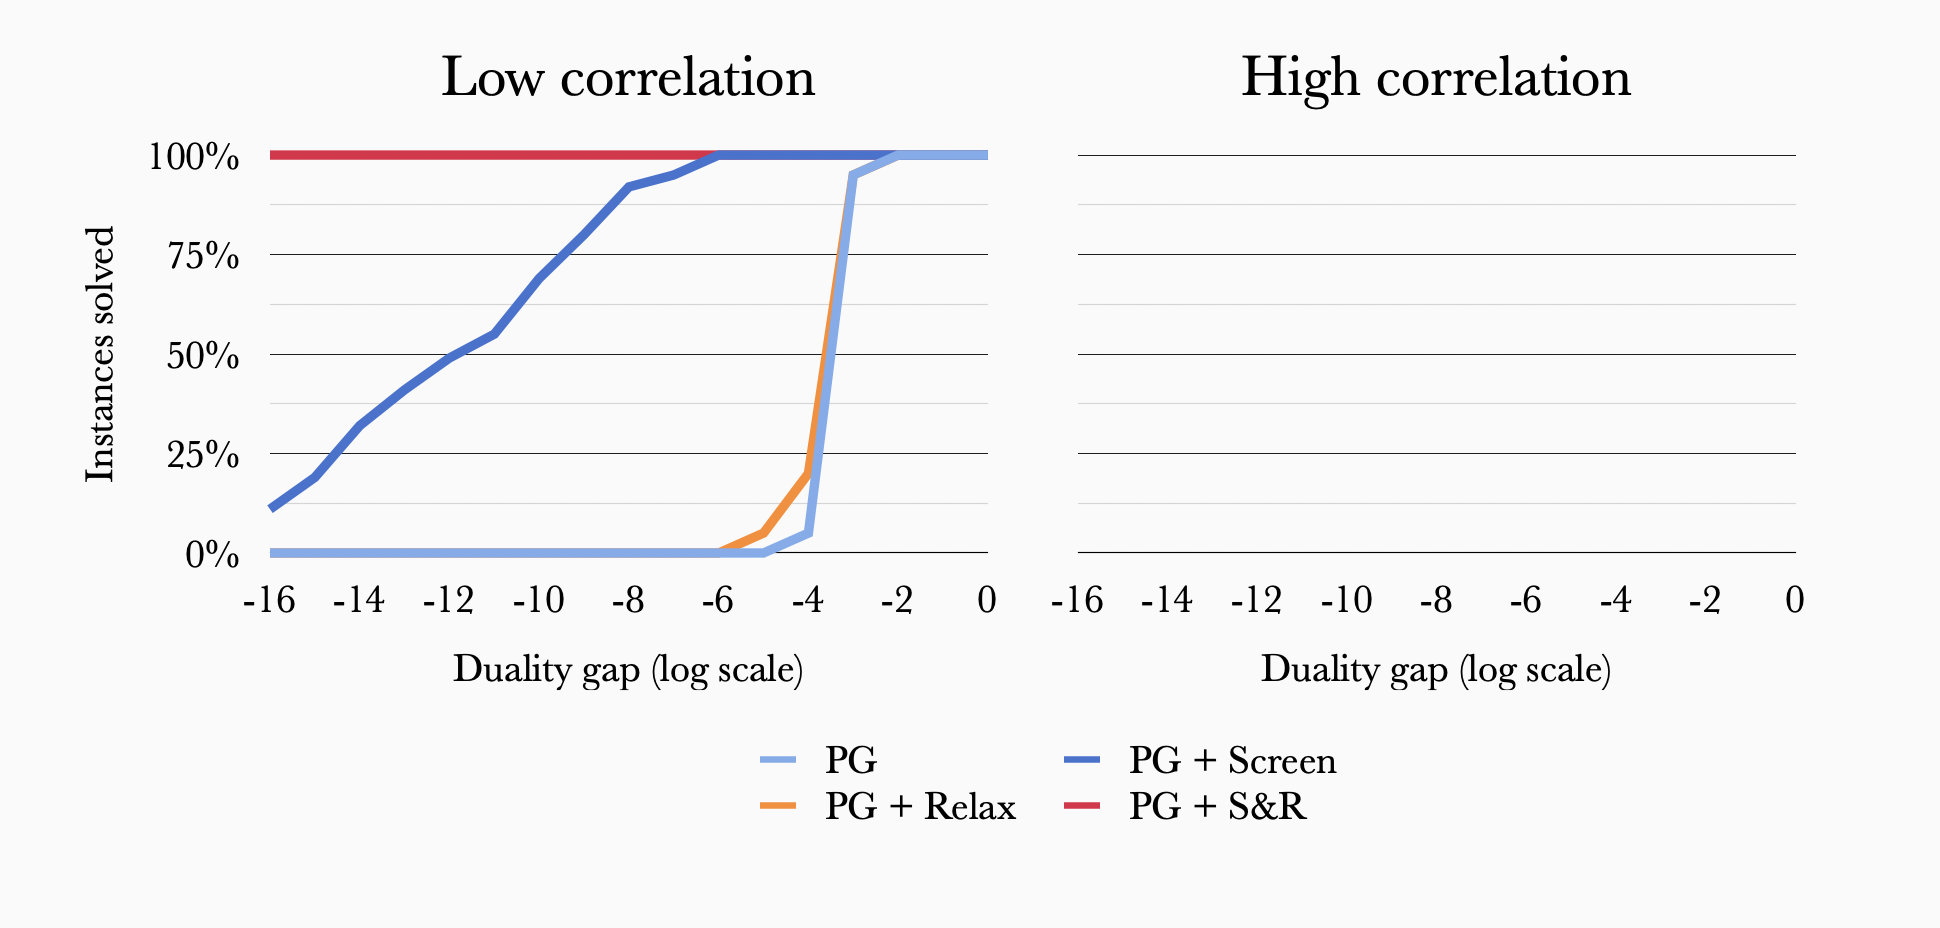
\includegraphics[width=\linewidth]{img/8.png}
  \end{figure}
\end{frame}

\begin{frame}{Some numerical results}
  \textbf{Setup :} Percentage of instances solved up to a given accuracy for a fixed FLOPs budget.
  \begin{figure}
    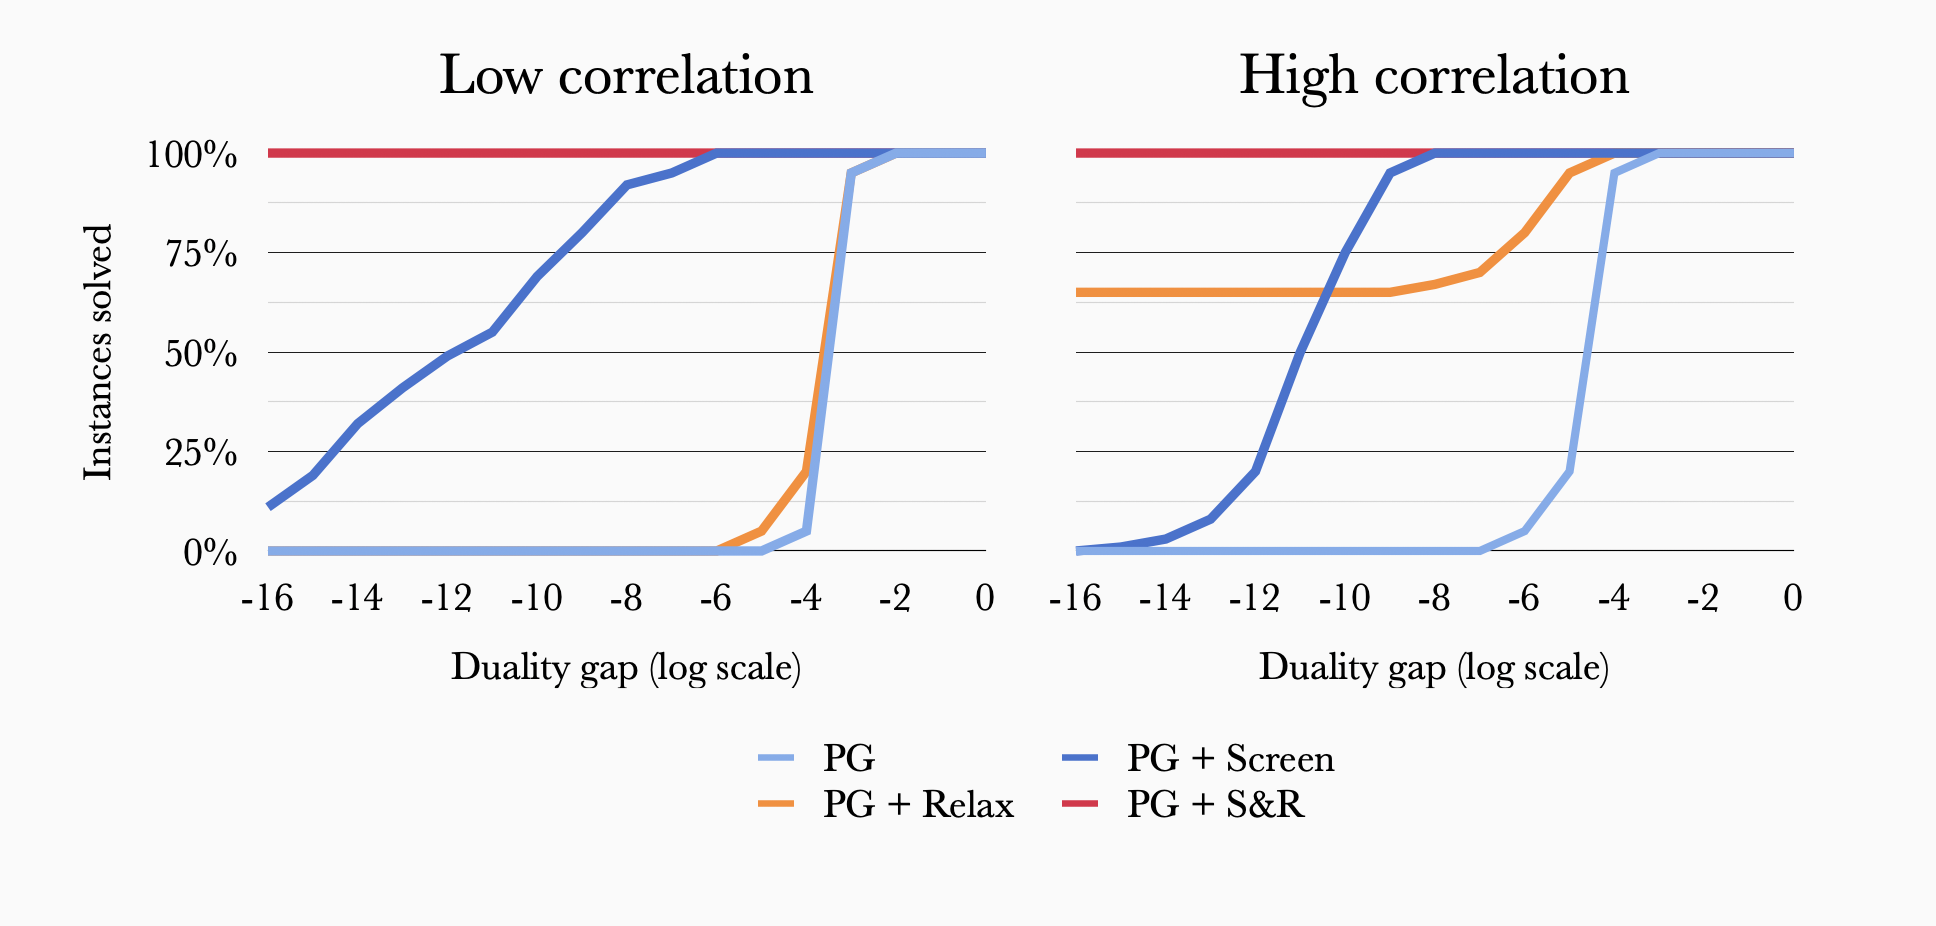
\includegraphics[width=\linewidth]{img/9.png}
  \end{figure}
\end{frame}

\end{document}
